\section{Lecture 5: The IMU Model and IMU Integration}
\label{sec:lecture05}

\subsection*{Topics}
\begin{itemize}[itemsep=0.3em]
\item the IMU measurement model (gyroscope, accelerometer, biases, noise);
\item continuous vs.\ discrete noise;
\item the IMU kinematics as a first-order ODE;
\item the big picture: IMU integration in a visual-inertial navigation system;
\item exact integration from $t_k$ to $t_{k+1}$;
\item computing $\Delta\vect{R},\Delta\vect{p},\Delta\vect{v}$ --- preintegration and three methods;
\item mean and covariance propagation with $SO(3)+\mathbb{R}^{3}$ errors;
\item the linearization using $SE_2(3)$.
\end{itemize}

% Tighten matrix column spacing for the dense block-matrix algebra in this lecture.
\setlength{\arraycolsep}{3.5pt}

% =====================================================================
\subsection{The IMU model}

The IMU (inertial measurement unit) is one of the most important sensors for robotics. We use two frames:
\begin{itemize}[noitemsep,topsep=2pt]
\item $\{I\}$: the IMU frame (attached to the sensor, see Fig.~\ref{fig:lec05-imu});
\item $\{G\}$: the global frame.
\end{itemize}
The IMU provides two readings: the \textbf{gyroscope} reads angular velocity and the \textbf{accelerometer} reads acceleration,
\begin{empheq}[box=\fbox]{align}
{}^{I}\vect{\omega}_{m} &= {}^{I}\vect{\omega} + \vect{b}_g + \vect{n}_g, \label{eq:lec05-gyro} \\
{}^{I}\vect{a}_{m} &= {}^{I}\vect{a} + \vect{b}_a + \vect{n}_a, \label{eq:lec05-accel}
\end{empheq}
where
\begin{itemize}[noitemsep,topsep=2pt]
\item ${}^{I}\vect{\omega}$ is the true angular-rate reading and ${}^{I}\vect{a}$ the true acceleration reading;
\item $\vect{b}_g$ is the gyro bias, driven by a random walk $\dot{\vect{b}}_g = \vect{n}_{wg}$; $\vect{b}_a$ is the accel bias, driven by a random walk $\dot{\vect{b}}_a = \vect{n}_{wa}$;
\item $\vect{n}_g \sim \mathcal{N}(\vect{0},\sigma_g^2\vect{I}_3)$ and $\vect{n}_a \sim \mathcal{N}(\vect{0},\sigma_a^2\vect{I}_3)$ are Gaussian noises.
\end{itemize}

\begin{figure}[H]
\centering
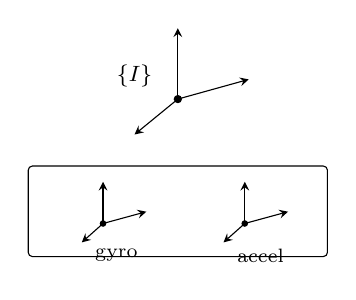
\begin{tikzpicture}[>=stealth]
  % IMU frame {I} above the body
  \fill (1.4,2.0) circle (1.5pt);
  \draw[->] (1.4,2.0) -- (1.4,2.9);
  \draw[->] (1.4,2.0) -- (2.3,2.25);
  \draw[->] (1.4,2.0) -- (0.85,1.55);
  \node at (0.85,2.30) {\footnotesize $\{I\}$};
  % IMU body containing the two sensors
  \draw[rounded corners=1.5pt] (-0.5,0) rectangle (3.3,1.15);
  % gyro triad
  \fill (0.45,0.42) circle (1.2pt);
  \draw[->] (0.45,0.42) -- (0.45,0.95);
  \draw[->] (0.45,0.42) -- (1.0,0.57);
  \draw[->] (0.45,0.42) -- (0.18,0.18);
  \node[below] at (0.62,0.22) {\scriptsize gyro};
  % accel triad
  \fill (2.25,0.42) circle (1.2pt);
  \draw[->] (2.25,0.42) -- (2.25,0.95);
  \draw[->] (2.25,0.42) -- (2.8,0.57);
  \draw[->] (2.25,0.42) -- (1.98,0.18);
  \node[below] at (2.45,0.22) {\scriptsize accel};
\end{tikzpicture}
\caption{The IMU carries its own frame $\{I\}$; onboard, the gyroscope reads the angular velocity and the accelerometer reads the acceleration.}
\label{fig:lec05-imu}
\end{figure}

\noindent Another way of modeling the accelerometer makes gravity explicit:
\begin{align}
{}^{I}\vect{a}_{m} = \big({}^{I}\vect{a}_b - {}^{I}_{G}\vect{R}\,{}^{G}\vect{g}\big) + \vect{b}_a + \vect{n}_a,
\qquad
{}^{G}\vect{g} = \begin{bmatrix} 0 \\ 0 \\ -9.8 \end{bmatrix},
\end{align}
where ${}^{I}\vect{a}_b$ is the body acceleration and ${}^{G}\vect{g}$ is gravity in $\{G\}$.

We use \eqref{eq:lec05-gyro} and \eqref{eq:lec05-accel} as our measurements. Inverting them gives the true readings:
\begin{align}
\text{true gyro reading:} \quad {}^{I}\vect{\omega} &= {}^{I}\vect{\omega}_{m} - \vect{b}_g - \vect{n}_g, \\
\text{true accel reading:} \quad {}^{I}\vect{a} &= {}^{I}\vect{a}_{m} - \vect{b}_a - \vect{n}_a.
\end{align}

\paragraph{The IMU state.} When we model the IMU, we use the following parameters:
\begin{itemize}[noitemsep,topsep=2pt]
\item $\{{}^{G}_{I}\vect{R}, {}^{G}\vect{p}_I\}$: IMU orientation and position --- 6 DoF;
\item ${}^{G}\vect{v}_I$: IMU velocity --- 3 DoF;
\item $\vect{b}_g$: gyro bias --- 3 DoF; \quad $\vect{b}_a$: accel bias --- 3 DoF.
\end{itemize}
Then our state vector for the IMU is
\begin{align}
\vect{x}_I = \big\{ {}^{G}_{I}\vect{R},\; {}^{G}\vect{p}_I,\; {}^{G}\vect{v}_I,\; \vect{b}_g,\; \vect{b}_a \big\}, \qquad \text{15 DoF}.
\end{align}
Some places use the quaternion ${}^{G}_{I}\vect{R} \Leftrightarrow {}^{G}_{I}\bar{q}$ (Lecture~2); then
\begin{align}
\vect{x}_I = \begin{bmatrix} {}^{G}_{I}\bar{q}\trans & {}^{G}\vect{p}_I\trans & {}^{G}\vect{v}_I\trans & \vect{b}_g\trans & \vect{b}_a\trans \end{bmatrix}\trans, \qquad 16\times1 \;\Rightarrow\; \text{15 DoF}.
\end{align}

% =====================================================================
\subsection{Continuous and discrete noise}

For the IMU we specify \emph{continuous-time} noise, $\vect{n}_c \sim \mathcal{N}(\vect{0},\sigma_c^2\vect{I}_3)$, characterized by
\begin{align}
\E\big[\vect{n}_c(t)\big] = \vect{0}_{3\times1}, \qquad
\E\big[\vect{n}_c(t+\tau)\,\vect{n}_c\trans(t)\big] = \sigma_c^2\vect{I}_3\,\delta(\tau),
\end{align}
where $\delta(\tau)$ is the impulse function: $\delta(\tau) = 1$ if $\tau = 0$ and $\delta(\tau) = 0$ if $\tau \neq 0$.

Consider a random-walk bias driven by this noise, $\dot{\vect{b}}(t) = \vect{n}_c(t)$. Integrating from $t_k$ to $t_{k+1}$,
\begin{align}
\int_{t_k}^{t_{k+1}} \dot{\vect{b}}(t)\,dt = \int_{t_k}^{t_{k+1}} \vect{n}_c(t)\,dt = \vect{b}_{k+1} - \vect{b}_k
\;\;\Rightarrow\;\;
\Delta\vect{b} \triangleq \vect{b}_{k+1} - \vect{b}_k = \int_{t_k}^{t_{k+1}} \vect{n}_c(t)\,dt.
\end{align}
Its mean is $\E(\Delta\vect{b}) = \E\big(\int_{t_k}^{t_{k+1}}\vect{n}_c(t)\,dt\big) = \vect{0}_{3\times1}$, and its covariance is
\begin{align}
\text{Cov}(\Delta\vect{b}) \triangleq \vect{P}_{\Delta\vect{b}}
= \E\big(\Delta\vect{b}\,\Delta\vect{b}\trans\big)
&= \E\left(\int_{t_k}^{t_{k+1}} \vect{n}_c(t)\,dt \cdot \int_{t_k}^{t_{k+1}} \vect{n}_c\trans(t)\,dt\right) \\
&= \E\left(\int_{t_k}^{t_{k+1}}\!\!\int_{t_k}^{t_{k+1}} \vect{n}_c(t)\,\vect{n}_c\trans(s)\,dt\,ds\right) \\
&= \int_{t_k}^{t_{k+1}} \E\big(\vect{n}_c(t)\,\vect{n}_c\trans(t)\big)\,dt \\
&= \int_{t_k}^{t_{k+1}} \sigma_c^2\vect{I}_3\,dt = \delta t\,\sigma_c^2\,\vect{I}_3,
\end{align}
where $\delta t = t_{k+1} - t_k$ (the impulse $\delta(\cdot)$ collapses the double integral). Hence we can \textbf{discretize} $\vect{n}_c$ in $[t_k,t_{k+1}]$ as
\begin{empheq}[box=\fbox]{align}
\vect{n}_d \sim \mathcal{N}\!\left(\vect{0},\,\frac{\sigma_c^2}{\delta t}\,\vect{I}_3\right), \qquad \delta t = t_{k+1} - t_k.
\end{empheq}
Then $\Delta\vect{b} = \int_{t_k}^{t_{k+1}} \vect{n}_c\,dt = \vect{n}_d\cdot\delta t$, and the discrete covariance is consistent with the continuous one:
\begin{align}
\text{Cov}(\Delta\vect{b})_d = \E\big(\vect{n}_d\vect{n}_d\trans\big)\,\delta t^2
= \delta t^2\cdot\frac{\sigma_c^2}{\delta t}\,\vect{I}_3
= \sigma_c^2\,\delta t\,\vect{I}_3
= \text{Cov}(\Delta\vect{b})_c. \checkmark
\end{align}

% =====================================================================
\subsection{The IMU kinematics: a first-order ODE}

The IMU state evolves by the first-order ordinary differential equation
\begin{align}
\begin{cases}
{}^{G}_{I}\dot{\vect{R}} = {}^{G}_{I}\vect{R}\,\skewsym{{}^{I}\vect{\omega}} = {}^{G}_{I}\vect{R}\,\skewsym{{}^{I}\vect{\omega}_m - \vect{b}_g - \vect{n}_g}, \\[3pt]
{}^{G}\dot{\vect{p}}_I = {}^{G}\vect{v}_I, \\[3pt]
{}^{G}\dot{\vect{v}}_I = {}^{G}\vect{a} + {}^{G}\vect{g} = {}^{G}_{I}\vect{R}\,\big({}^{I}\vect{a}_m - \vect{b}_a - \vect{n}_a\big) + {}^{G}\vect{g}, \\[3pt]
{}^{I}\dot{\vect{b}}_g = \vect{n}_{wg}, \qquad {}^{I}\dot{\vect{b}}_a = \vect{n}_{wa}.
\end{cases}
\end{align}
Stacking, we obtain the compact form
\begin{empheq}[box=\fbox]{align}
\dot{\vect{x}}_I = \vect{f}(\vect{x}_I, \vect{n}_I), \qquad
\vect{n}_I = \begin{bmatrix} \vect{n}_g \\ \vect{n}_a \\ \vect{n}_{wg} \\ \vect{n}_{wa} \end{bmatrix},
\quad
\begin{aligned}
\vect{n}_g &\sim \mathcal{N}(\vect{0},\sigma_g^2\vect{I}_3), & \vect{n}_a &\sim \mathcal{N}(\vect{0},\sigma_a^2\vect{I}_3), \\
\vect{n}_{wg} &\sim \mathcal{N}(\vect{0},\sigma_{wg}^2\vect{I}_3), & \vect{n}_{wa} &\sim \mathcal{N}(\vect{0},\sigma_{wa}^2\vect{I}_3),
\end{aligned}
\label{eq:lec05-ode}
\end{empheq}
and, per the previous subsection, the discretized noise over one interval is
\begin{align}
\vect{n}_{Id} = \begin{bmatrix} \vect{n}_{gd} \\ \vect{n}_{ad} \\ \vect{n}_{wgd} \\ \vect{n}_{wad} \end{bmatrix},
\qquad
\sigma_{gd}^2 = \frac{\sigma_g^2}{\delta t}, \quad
\sigma_{ad}^2 = \frac{\sigma_a^2}{\delta t}, \quad
\sigma_{wgd}^2 = \frac{\sigma_{wg}^2}{\delta t}, \quad
\sigma_{wad}^2 = \frac{\sigma_{wa}^2}{\delta t}.
\end{align}
The IMU model is done. There are various IMU models, but the basic idea is the same.

% =====================================================================
\subsection{IMU integration: the big picture}

Recall the typical linear system from Lecture~1 and put it side by side with our sensor models (Fig.~\ref{fig:lec05-vins}):
\begin{align}
\begin{cases}
\dot{\vect{x}} = \vect{A}\vect{x} + \vect{B}\vect{u} & \to \text{state evolution} \to \text{IMU model:} \quad \dot{\vect{x}}_I = \vect{f}(\vect{x}_I,\vect{n}_I), \\[2pt]
\vect{y} = \vect{C}\vect{x} + \vect{D}\vect{u} & \to \text{observation / measurements} \to \text{vision / camera model:} \quad \vect{z}_c = \vect{h}_c(\vect{x}) + \vect{n}_c.
\end{cases}
\end{align}
Together they form a \textbf{VINS} (visual-inertial navigation system). These two models are the focus of our tutorials: how to process the camera measurement $\vect{z}_c = \vect{h}_c(\vect{x})+\vect{n}_c$ was covered in Lectures~3 and~4; we will learn how to process the IMU in this Lecture~5.

\begin{figure}[H]
\centering
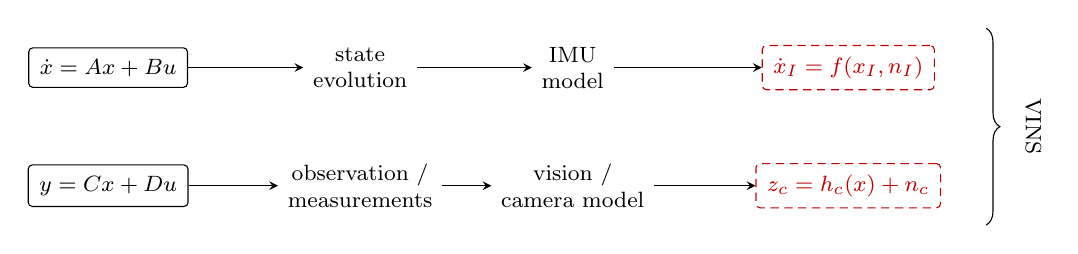
\begin{tikzpicture}[>=stealth,
  box/.style={draw,rounded corners=1.5pt,inner sep=4pt,align=center,font=\footnotesize},
  lbl/.style={font=\footnotesize,align=center}]
  % top row: state evolution -> IMU
  \node[box] (lin1) at (0,1.5) {$\dot{\vect{x}} = \vect{A}\vect{x}+\vect{B}\vect{u}$};
  \node[lbl] (se) at (3.2,1.5) {state\\evolution};
  \node[lbl] (im) at (5.9,1.5) {IMU\\model};
  \node[box,densely dashed,red!75!black] (eq3) at (9.4,1.5) {$\dot{\vect{x}}_I = \vect{f}(\vect{x}_I,\vect{n}_I)$};
  \draw[->] (lin1) -- (se); \draw[->] (se) -- (im); \draw[->] (im) -- (eq3);
  % bottom row: observation -> camera
  \node[box] (lin2) at (0,0) {$\vect{y} = \vect{C}\vect{x}+\vect{D}\vect{u}$};
  \node[lbl] (ob) at (3.2,0) {observation /\\measurements};
  \node[lbl] (cm) at (5.9,0) {vision /\\camera model};
  \node[box,densely dashed,red!75!black] (eq4) at (9.4,0) {$\vect{z}_c = \vect{h}_c(\vect{x})+\vect{n}_c$};
  \draw[->] (lin2) -- (ob); \draw[->] (ob) -- (cm); \draw[->] (cm) -- (eq4);
  % VINS brace
  \draw[decorate,decoration={brace,amplitude=5pt}] (11.15,2.0) -- (11.15,-0.5);
  \node[lbl,rotate=-90] at (11.75,0.75) {VINS};
\end{tikzpicture}
\caption{The big picture: the Lecture-1 linear system maps onto the two VINS models --- the IMU model plays the state evolution (this lecture) and the camera model plays the observation (Lectures~3--4).}
\label{fig:lec05-vins}
\end{figure}

\paragraph{The problem formulation.} Given $\vect{x}_k \sim \mathcal{N}(\hat{\vect{x}}_k, \vect{P}_k)$ and the IMU readings $({}^{I}\vect{\omega}_{m_k}, {}^{I}\vect{a}_{m_k})$, solve
\begin{empheq}[box=\fbox]{align}
\vect{x}_{k+1} \sim \mathcal{N}(\hat{\vect{x}}_{k+1}, \vect{P}_{k+1})
\quad\Rightarrow\quad
\text{two targets:}\;\; \hat{\vect{x}}_{k+1} \;\text{and}\; \vect{P}_{k+1}.
\end{empheq}
That is, the ODE $\dot{\vect{x}}_I = \vect{f}(\vect{x}_I,\vect{n}_I)$ carries the \emph{current state distribution} $\vect{x}_k \sim \mathcal{N}(\hat{\vect{x}}_k,\vect{P}_k)$ into the \emph{next state distribution} $\vect{x}_{k+1} \sim \mathcal{N}(\hat{\vect{x}}_{k+1},\vect{P}_{k+1})$.

\paragraph{How to solve it?} From $\dot{\vect{x}}_I = \vect{f}(\vect{x}_I,\vect{n}_I)$ we can get the \emph{integrated function}
\begin{align}
\vect{x}_{k+1} = \vect{f}_{\mathrm{int}}\big(\vect{x}_k,\, {}^{I}\vect{\omega}_m,\, {}^{I}\vect{a}_m,\, \vect{n}_k\big),
\qquad
\begin{cases}
\vect{x}_{k+1} = \vect{x}_{I_{k+1}}, \\
\vect{x}_{k} = \vect{x}_{I_{k}}, \\
\vect{n}_{k} = \vect{n}_{I_k} \sim \mathcal{N}(\vect{0}, \vect{R}_{I_k}).
\end{cases}
\end{align}
Hence the \textbf{mean} is propagated with zero noise,
\begin{align}
\hat{\vect{x}}_{k+1} = \vect{f}_{\mathrm{int}}\big(\hat{\vect{x}}_k,\, {}^{I}\vect{\omega}_m,\, {}^{I}\vect{a}_m,\, \vect{0}\big)
\quad\to\quad \text{solved } \hat{\vect{x}}_{k+1}.
\end{align}
Then, linearizing $\vect{f}_{\mathrm{int}}$, we get the error-state propagation with the discretized noise $\vect{n}_{kd}$,
\begin{align}
\tilde{\vect{x}}_{k+1} = \vect{\Phi}_{(k+1,k)}\,\tilde{\vect{x}}_k + \vect{G}_k\,\vect{n}_{kd},
\end{align}
and therefore the \textbf{covariance}
\begin{align}
\vect{P}_{k+1} = \E\big(\tilde{\vect{x}}_{k+1}\tilde{\vect{x}}_{k+1}\trans\big)
= \vect{\Phi}_{(k+1,k)}\,\vect{P}_k\,\vect{\Phi}_{(k+1,k)}\trans + \vect{G}_k\,\vect{R}_{Id}\,\vect{G}_k\trans
\quad\to\quad \text{solved } \vect{P}_{k+1}.
\end{align}
Given the big picture, let's explore the detailed derivations.

% =====================================================================
\subsection{Exact integration from \texorpdfstring{$t_k$ to $t_{k+1}$}{tk to tk+1}}
\label{sec:lec05-exact}

\paragraph{The input.} Split each true reading into its estimate and error,
\begin{align}
{}^{I}\vect{\omega} = {}^{I}\vect{\omega}_m - \vect{b}_g - \vect{n}_g
= \underbrace{\big({}^{I}\vect{\omega}_m - \hat{\vect{b}}_g\big)}_{{}^{I}\hat{\vect{\omega}}}
+ \underbrace{\big(-\tilde{\vect{b}}_g - \vect{n}_g\big)}_{{}^{I}\tilde{\vect{\omega}}}
= {}^{I}\hat{\vect{\omega}} + {}^{I}\tilde{\vect{\omega}}, \\
{}^{I}\vect{a} = {}^{I}\vect{a}_m - \vect{b}_a - \vect{n}_a
= \underbrace{\big({}^{I}\vect{a}_m - \hat{\vect{b}}_a\big)}_{{}^{I}\hat{\vect{a}}}
+ \underbrace{\big(-\tilde{\vect{b}}_a - \vect{n}_a\big)}_{{}^{I}\tilde{\vect{a}}}
= {}^{I}\hat{\vect{a}} + {}^{I}\tilde{\vect{a}}.
\end{align}
We integrate from $k$ to $k+1$, with $\delta t = t_{k+1} - t_k$.

\paragraph{For rotation.}
\begin{align}
{}^{G}_{I_{k+1}}\vect{R} = {}^{G}_{I_{k}}\vect{R}\cdot{}^{I_k}_{I_{k+1}}\vect{R}, \qquad
\Delta\vect{R} \triangleq {}^{I_k}_{I_{k+1}}\vect{R},
\end{align}
where $\Delta\vect{R}$ is the rotation integration from ${}^{I}\vect{\omega}$.

\paragraph{For velocity.} From ${}^{G}\dot{\vect{v}}_{I_\tau} = {}^{G}_{I_\tau}\vect{R}\,{}^{I_\tau}\vect{a} + {}^{G}\vect{g}$,
\begin{align}
\int_{t_k}^{t_{k+1}} {}^{G}\dot{\vect{v}}_{I_\tau}\,d\tau
= \int_{t_k}^{t_{k+1}} \big({}^{G}_{I_\tau}\vect{R}\,{}^{I_\tau}\vect{a} + {}^{G}\vect{g}\big)\,d\tau.
\end{align}
The left-hand side is $\int_{t_k}^{t_{k+1}} {}^{G}\dot{\vect{v}}_{I_\tau}\,d\tau = {}^{G}\vect{v}_{I_{k+1}} - {}^{G}\vect{v}_{I_k}$, and the right-hand side is
\begin{align}
\int_{t_k}^{t_{k+1}} \big({}^{G}_{I_\tau}\vect{R}\,{}^{I_\tau}\vect{a} + {}^{G}\vect{g}\big)\,d\tau
&= \int_{t_k}^{t_{k+1}} {}^{G}_{I_\tau}\vect{R}\,{}^{I_\tau}\vect{a}\,d\tau + {}^{G}\vect{g}\,\delta t \\
&= \int_{t_k}^{t_{k+1}} {}^{G}_{I_k}\vect{R}\,{}^{I_k}_{I_\tau}\vect{R}\,{}^{I_\tau}\vect{a}\,d\tau + {}^{G}\vect{g}\,\delta t \\
&= {}^{G}_{I_k}\vect{R} \underbrace{\int_{t_k}^{t_{k+1}} {}^{I_k}_{I_\tau}\vect{R}\,{}^{I_\tau}\vect{a}\,d\tau}_{\Delta\vect{v}} + {}^{G}\vect{g}\,\delta t.
\end{align}
Then
\begin{align}
{}^{G}\vect{v}_{I_{k+1}} = {}^{G}\vect{v}_{I_k} + {}^{G}_{I_k}\vect{R}\,\Delta\vect{v} + {}^{G}\vect{g}\,\delta t,
\qquad
\Delta\vect{v} \triangleq \int_{t_k}^{t_{k+1}} {}^{I_k}_{I_\tau}\vect{R}\,{}^{I_\tau}\vect{a}\,d\tau,
\end{align}
where $\Delta\vect{v}$ is the integration of ${}^{I}\vect{\omega}$ and ${}^{I}\vect{a}$.

\paragraph{For position.} From ${}^{G}\dot{\vect{p}}_{I_\tau} = {}^{G}\vect{v}_{I_\tau}$,
\begin{align}
\int_{t_k}^{t_{k+1}} {}^{G}\dot{\vect{p}}_{I_\tau}\,d\tau = \int_{t_k}^{t_{k+1}} {}^{G}\vect{v}_{I_\tau}\,d\tau.
\end{align}
Note that, by the velocity result applied up to time $\tau$ (with $\delta\tau = \tau - t_k$),
\begin{align}
{}^{G}\vect{v}_{I_\tau} = {}^{G}\vect{v}_{I_k} + {}^{G}_{I_k}\vect{R}\int_{t_k}^{\tau} {}^{I_k}_{I_s}\vect{R}\,{}^{I_s}\vect{a}\,ds + {}^{G}\vect{g}\,\delta\tau.
\end{align}
The left-hand side is ${}^{G}\vect{p}_{I_{k+1}} - {}^{G}\vect{p}_{I_k}$, and the right-hand side becomes
\begin{align}
\int_{t_k}^{t_{k+1}} {}^{G}\vect{v}_{I_\tau}\,d\tau
&= \int_{t_k}^{t_{k+1}} \left( {}^{G}\vect{v}_{I_k} + {}^{G}_{I_k}\vect{R}\int_{t_k}^{\tau} {}^{I_k}_{I_s}\vect{R}\,{}^{I_s}\vect{a}\,ds + {}^{G}\vect{g}\,\delta\tau \right) d\tau \\
&= \int_{t_k}^{t_{k+1}} {}^{G}\vect{v}_{I_k}\,d\tau + \int_{t_k}^{t_{k+1}} {}^{G}\vect{g}\,\delta\tau\,d\tau + {}^{G}_{I_k}\vect{R}\int_{t_k}^{t_{k+1}}\!\!\int_{t_k}^{\tau} {}^{I_k}_{I_s}\vect{R}\,{}^{I_s}\vect{a}\,ds\,d\tau \\
&= {}^{G}\vect{v}_{I_k}\,\delta t + \frac{1}{2}{}^{G}\vect{g}\,\delta t^2 + {}^{G}_{I_k}\vect{R}\underbrace{\int_{t_k}^{t_{k+1}}\!\!\int_{t_k}^{\tau} {}^{I_k}_{I_s}\vect{R}\,{}^{I_s}\vect{a}\,ds\,d\tau}_{\Delta\vect{p}}.
\end{align}
Then
\begin{align}
{}^{G}\vect{p}_{I_{k+1}} = {}^{G}\vect{p}_{I_k} + {}^{G}\vect{v}_{I_k}\,\delta t + {}^{G}_{I_k}\vect{R}\,\Delta\vect{p} + \frac{1}{2}{}^{G}\vect{g}\,\delta t^2,
\qquad
\Delta\vect{p} \triangleq \int_{t_k}^{t_{k+1}}\!\!\int_{t_k}^{\tau} {}^{I_k}_{I_s}\vect{R}\,{}^{I_s}\vect{a}\,ds\,d\tau,
\end{align}
where $\Delta\vect{p}$ is the \emph{double} integration of ${}^{I}\vect{\omega}$ and ${}^{I}\vect{a}$.

\paragraph{For the biases.} From $\dot{\vect{b}}_g = \vect{n}_{wg}$,
\begin{align}
\int_{t_k}^{t_{k+1}} \dot{\vect{b}}_g\,d\tau = \int_{t_k}^{t_{k+1}} \vect{n}_{wg}\,d\tau
\;\;\Rightarrow\;\;
\vect{b}_{g_{k+1}} = \vect{b}_{g_k} + \int_{t_k}^{t_{k+1}} \vect{n}_{wg}\,d\tau,
\end{align}
and for the accel bias, $\vect{b}_{a_{k+1}} = \vect{b}_{a_k} + \int_{t_k}^{t_{k+1}} \vect{n}_{wa}\,d\tau$.

\paragraph{Finally.} Collecting everything:
\begin{empheq}[box=\fbox]{align}
{}^{G}_{I_{k+1}}\vect{R} &= {}^{G}_{I_k}\vect{R}\cdot\Delta\vect{R},
& \Delta\vect{R} &= {}^{I_k}_{I_{k+1}}\vect{R}, \notag \\
{}^{G}\vect{p}_{I_{k+1}} &= {}^{G}\vect{p}_{I_k} + {}^{G}\vect{v}_{I_k}\,\delta t + {}^{G}_{I_k}\vect{R}\,\Delta\vect{p} + \tfrac{1}{2}{}^{G}\vect{g}\,\delta t^2,
& \Delta\vect{p} &= \int_{t_k}^{t_{k+1}}\!\!\int_{t_k}^{\tau} {}^{I_k}_{I_s}\vect{R}\,{}^{I_s}\vect{a}\,ds\,d\tau, \notag \\
{}^{G}\vect{v}_{I_{k+1}} &= {}^{G}\vect{v}_{I_k} + {}^{G}_{I_k}\vect{R}\,\Delta\vect{v} + {}^{G}\vect{g}\,\delta t,
& \Delta\vect{v} &= \int_{t_k}^{t_{k+1}} {}^{I_k}_{I_\tau}\vect{R}\,{}^{I_\tau}\vect{a}\,d\tau, \label{eq:lec05-exact} \\
\vect{b}_{g_{k+1}} &= \vect{b}_{g_k} + \textstyle\int_{t_k}^{t_{k+1}} \vect{n}_{wg}\,d\tau,
& \Delta\vect{b}_g &= \int_{t_k}^{t_{k+1}} \vect{n}_{wg}\,d\tau, \notag \\
\vect{b}_{a_{k+1}} &= \vect{b}_{a_k} + \textstyle\int_{t_k}^{t_{k+1}} \vect{n}_{wa}\,d\tau,
& \Delta\vect{b}_a &= \int_{t_k}^{t_{k+1}} \vect{n}_{wa}\,d\tau. \notag
\end{empheq}
This is exactly the integrated function $\vect{x}_{k+1} = \vect{f}_{\mathrm{int}}(\vect{x}_k, {}^{I}\vect{\omega}_m, {}^{I}\vect{a}_m, \vect{n}_k)$.

\begin{quote}
\textbf{To this step, no assumption or approximation is made --- every step is accurate.} The accuracy of the integration is decided by how $\Delta\vect{R}$, $\Delta\vect{p}$, $\Delta\vect{v}$ are computed from ${}^{I}\vect{\omega}$ and ${}^{I}\vect{a}$.
\end{quote}

% =====================================================================
\subsection{Computing \texorpdfstring{$\Delta\vect{R},\Delta\vect{p},\Delta\vect{v}$}{dR, dp, dv}: preintegration and three methods}

The way to compute $\Delta\vect{R}$, $\Delta\vect{p}$, $\Delta\vect{v}$ given $\vect{\omega}_m$ and $\vect{a}_m$ defines the algorithms. A few discussions follow.

\paragraph{(1) Connection to preintegration.} $\Delta\vect{R}$, $\Delta\vect{p}$, $\Delta\vect{v}$ are also called the \emph{pre-integrated measurements}: they are only affected by ${}^{I}\vect{\omega}_m$, ${}^{I}\vect{a}_m$ and $\vect{b}_g$, $\vect{b}_a$ (not by the global state). Inverting \eqref{eq:lec05-exact},
\begin{align}
\Delta\vect{R} &\triangleq {}^{I_k}_{I_{k+1}}\vect{R}
&&= {}^{G}_{I_k}\vect{R}\trans\,{}^{G}_{I_{k+1}}\vect{R}, \\
\Delta\vect{p} &\triangleq \int_{t_k}^{t_{k+1}}\!\!\int_{t_k}^{\tau} {}^{I_k}_{I_s}\vect{R}\,{}^{I_s}\vect{a}\,ds\,d\tau
&&= {}^{G}_{I_k}\vect{R}\trans\big({}^{G}\vect{p}_{I_{k+1}} - {}^{G}\vect{p}_{I_k} - {}^{G}\vect{v}_{I_k}\,\delta t - \tfrac{1}{2}{}^{G}\vect{g}\,\delta t^2\big), \\
\Delta\vect{v} &\triangleq \int_{t_k}^{t_{k+1}} {}^{I_k}_{I_\tau}\vect{R}\,{}^{I_\tau}\vect{a}\,d\tau
&&= {}^{G}_{I_k}\vect{R}\trans\big({}^{G}\vect{v}_{I_{k+1}} - {}^{G}\vect{v}_{I_k} - {}^{G}\vect{g}\,\delta t\big), \\
\Delta\vect{b}_g &\triangleq \int_{t_k}^{t_{k+1}} \vect{n}_{wg}\,d\tau
&&= \vect{b}_{g_{k+1}} - \vect{b}_{g_k}, \\
\Delta\vect{b}_a &\triangleq \int_{t_k}^{t_{k+1}} \vect{n}_{wa}\,d\tau
&&= \vect{b}_{a_{k+1}} - \vect{b}_{a_k}.
\end{align}
So the IMU integration/propagation and pre-integration are connected: they compute the same quantities.

\paragraph{(2) Discrete preintegration on the manifold.} For example, IMU preintegration on manifold (Forster, Carlone, et al.)~\cite{Forster2017tro} and VINS-Mono (Tong Qin, Shaojie Shen)~\cite{Qin2017TRO}. Assume ${}^{I_k}\vect{\omega}$ and ${}^{I_k}\vect{a}$ are constant in $[t_k, t_{k+1}]$ \emph{and} $\delta t = t_{k+1} - t_k$ is small, so ${}^{I_k}_{I_\tau}\vect{R} \approx \vect{I}$ as $\delta t \to 0$:
\begin{align}
\Delta\vect{R} &\triangleq {}^{I_k}_{I_{k+1}}\vect{R} \approx \Exp\big({}^{I_k}\vect{\omega}\cdot\delta t\big), \\
\Delta\vect{p} &= \int_{t_k}^{t_{k+1}}\!\!\int_{t_k}^{\tau} {}^{I_k}_{I_s}\vect{R}\,{}^{I_s}\vect{a}\,ds\,d\tau
\approx \int_{t_k}^{t_{k+1}}\!\!\int_{t_k}^{\tau} \vect{I}_3\cdot{}^{I_k}\vect{a}\,ds\,d\tau
= \frac{1}{2}\,{}^{I_k}\vect{a}\,\delta t^2, \\
\Delta\vect{v} &= \int_{t_k}^{t_{k+1}} {}^{I_k}_{I_\tau}\vect{R}\,{}^{I_\tau}\vect{a}\,d\tau
\approx {}^{I_k}\vect{a}\,\delta t.
\end{align}
Then the propagation becomes
\begin{align}
\begin{cases}
{}^{G}_{I_{k+1}}\vect{R} = {}^{G}_{I_k}\vect{R}\cdot\Exp\big({}^{I_k}\vect{\omega}\,\delta t\big), \\[2pt]
{}^{G}\vect{p}_{I_{k+1}} = {}^{G}\vect{p}_{I_k} + {}^{G}\vect{v}_{I_k}\,\delta t + \frac{1}{2}\,{}^{G}_{I_k}\vect{R}\,{}^{I_k}\vect{a}\,\delta t^2 + \frac{1}{2}\,{}^{G}\vect{g}\,\delta t^2, \\[2pt]
{}^{G}\vect{v}_{I_{k+1}} = {}^{G}\vect{v}_{I_k} + {}^{G}_{I_k}\vect{R}\,{}^{I_k}\vect{a}\,\delta t + {}^{G}\vect{g}\,\delta t, \\[2pt]
\vect{b}_{g_{k+1}} = \vect{b}_{g_k} + \int_{t_k}^{t_{k+1}}\vect{n}_{wg}\,d\tau, \qquad
\vect{b}_{a_{k+1}} = \vect{b}_{a_k} + \int_{t_k}^{t_{k+1}}\vect{n}_{wa}\,d\tau.
\end{cases}
\end{align}
This is easy and simple, but it might lose some accuracy for fast rotation and low sampling rate ($\delta t$ larger).

\paragraph{(3) Analytic integration: ACI\textsuperscript{2} and CPI.} ACI$^2$ --- analytic combined IMU integration (Yulin/Chuchu)~\cite{Yang2020ACI2}; CPI --- continuous preintegration (Kevin/Patrick)~\cite{Eckenhoff2019IJRR,Eckenhoff2017ICRA}. If we assume only that ${}^{I_k}\vect{\omega}$ and ${}^{I_k}\vect{a}$ are constant in $[t_k, t_{k+1}]$ (without the small-$\delta t$ approximation), then ${}^{I_k}_{I_\tau}\vect{R} = \Exp({}^{I_k}\vect{\omega}\,\delta\tau)$ and
\begin{align}
\Delta\vect{R} &\triangleq {}^{I_k}_{I_{k+1}}\vect{R} = \Exp\big({}^{I_k}\vect{\omega}\cdot\delta t\big), \\
\Delta\vect{p} &= \int_{t_k}^{t_{k+1}}\!\!\int_{t_k}^{\tau} {}^{I_k}_{I_s}\vect{R}\,{}^{I_s}\vect{a}\,ds\,d\tau
= \int_{t_k}^{t_{k+1}}\!\!\int_{t_k}^{\tau} \Exp\big({}^{I_k}\vect{\omega}\,\delta s\big)\,{}^{I_k}\vect{a}\,ds\,d\tau, \\
\Delta\vect{v} &= \int_{t_k}^{t_{k+1}} {}^{I_k}_{I_\tau}\vect{R}\,{}^{I_\tau}\vect{a}\,d\tau
= \int_{t_k}^{t_{k+1}} \Exp\big({}^{I_k}\vect{\omega}\,\delta\tau\big)\,{}^{I_k}\vect{a}\,d\tau,
\end{align}
which admit closed-form (analytic) solutions.

\paragraph{(4) Two ways to solve for $\hat{\vect{x}}_{k+1}$ and $\vect{P}_{k+1}$.} We can use different ways to solve for $\hat{\vect{x}}_{k+1}$ and $\vect{P}_{k+1}$.

\emph{Way 1 --- discretize, then linearize.} Integrate the nonlinear ODE first, then linearize the integrated function (the route taken in this lecture):
\begin{align}
\dot{\vect{x}} = \vect{f}(\vect{x},\vect{n}_I)
\;\;\to\;\;
\vect{x}_{k+1} = \vect{f}_{\mathrm{int}}(\vect{x}_k,\vect{n}_k)
\;\;\to\;\;
\begin{cases}
\hat{\vect{x}}_{k+1} = \vect{f}_{\mathrm{int}}(\hat{\vect{x}}_k,\vect{0}), \\[2pt]
\tilde{\vect{x}}_{k+1} = \vect{\Phi}_{(k+1,k)}\,\tilde{\vect{x}}_k + \vect{G}_k\,\vect{n}_{kd}.
\end{cases}
\end{align}

\emph{Way 2 --- linearize, then integrate.} Linearize the continuous ODE first to get the continuous error-state equation, then integrate it:
\begin{align}
\dot{\vect{x}} = \vect{f}(\vect{x},\vect{n}_I)
\;\;\Rightarrow\;\;
\dot{\tilde{\vect{x}}} = \vect{F}\,\tilde{\vect{x}} + \vect{J}\,\vect{n}_I,
\end{align}
whose solution over $[t_k,t_{k+1}]$ is
\begin{align}
\tilde{\vect{x}}_{k+1} = \vect{\Phi}_{(k+1,k)}\,\tilde{\vect{x}}_k + \int_{t_k}^{t_{k+1}} \vect{\Phi}_{(k+1,\tau)}\,\vect{J}(\tau)\,\vect{n}_I\,d\tau,
\qquad
\vect{\Phi}_{(k+1,k)} = \exp\!\left(\int_{t_k}^{t_{k+1}} \vect{F}\,dt\right).
\label{eq:lec05-way2}
\end{align}
Different systems treat this state-transition matrix differently:
\begin{itemize}[noitemsep,topsep=2pt]
\item \textbf{VINS-Mono}~\cite{Qin2017TRO}: take $\vect{F}$ constant and $\delta t \to 0$, so
$\vect{\Phi}_{(k+1,k)} = \exp\big(\int_{t_k}^{t_{k+1}}\vect{F}\,dt\big) \approx \vect{I} + \vect{F}\,\delta t$;
\item \textbf{OC-VINS} (Joel Hesch)~\cite{Hesch2013TRO} / \textbf{CPI} (Kevin/Patrick)~\cite{Eckenhoff2019IJRR} / \textbf{ACI$^2$} (Yulin/Chuchu)~\cite{Yang2020ACI2}: keep
$\vect{\Phi}_{(k+1,k)} = \exp\big(\int_{t_k}^{t_{k+1}}\vect{F}\,dt\big)$, evaluated with ${}^{I}\vect{\omega}_m$, ${}^{I}\vect{a}_m$ constant in $[t_k,t_{k+1}]$.
\end{itemize}
How to address the noise term of \eqref{eq:lec05-way2},
\begin{align}
\vect{n}_{\mathrm{int}} \triangleq \int_{t_k}^{t_{k+1}} \vect{\Phi}_{(k+1,\tau)}\,\vect{J}(\tau)\,\vect{n}_I\,d\tau\,?
\end{align}
\begin{enumerate}[label=(\arabic*),noitemsep,topsep=2pt]
\item Pull the \emph{discrete noise} $\vect{n}_{Id}$ out of the integral:
\begin{align}
\vect{n}_{\mathrm{int}} &= \int_{t_k}^{t_{k+1}} \vect{\Phi}_{(k+1,\tau)}\,\vect{J}(\tau)\,d\tau\cdot\vect{n}_{Id}, \\
\Rightarrow\;
\text{Cov}(\vect{n}_{\mathrm{int}}) &= \int_{t_k}^{t_{k+1}} \vect{\Phi}_{(k+1,\tau)}\vect{J}(\tau)\,d\tau
\cdot \vect{Q}_{Id} \cdot
\left(\int_{t_k}^{t_{k+1}} \vect{\Phi}_{(k+1,\tau)}\vect{J}(\tau)\,d\tau\right)^{\!\top}\!.
\end{align}
\item Keep the noise inside the integral:
\begin{align}
\text{Cov}(\vect{n}_{\mathrm{int}})
&= \E\left(\int_{t_k}^{t_{k+1}} \vect{\Phi}_{(k+1,\tau)}\,\vect{J}(\tau)\,\vect{n}_{Id}\,\vect{n}_{Id}\trans\,\vect{J}\trans(\tau)\,\vect{\Phi}_{(k+1,\tau)}\trans\,d\tau\right) \\
&= \int_{t_k}^{t_{k+1}} \vect{\Phi}_{(k+1,\tau)}\,\vect{J}(\tau)\,\vect{Q}_{Id}\,\vect{J}\trans(\tau)\,\vect{\Phi}_{(k+1,\tau)}\trans\,d\tau.
\end{align}
\end{enumerate}
Either way, the \emph{linearization} itself can be carried out with different error parametrizations, all 15~DoF for $\vect{x}_I$:
\begin{empheq}[box=\fbox]{align}
\begin{cases}
SO(3) + \mathbb{R}^3 + \mathbb{R}^3 + \mathbb{R}^3 + \mathbb{R}^3 &\Rightarrow\; \text{15 DoF for } \vect{x}_I, \\
SE_2(3) + \mathbb{R}^3 + \mathbb{R}^3 &\Rightarrow\; \text{15 DoF for } \vect{x}_I, \\
SE(3) + \mathbb{R}^3 + \mathbb{R}^3 + \mathbb{R}^3 &\Rightarrow\; \text{15 DoF for } \vect{x}_I.
\end{cases}
\end{empheq}
We now use the analytic form from (3) for the detailed mean and covariance propagation, working out the first two parametrizations: $SO(3)+\mathbb{R}^{12}$ in \S\ref{sec:lec05-so3prop} and $SE_2(3)+\mathbb{R}^{6}$ in the final subsection.

% =====================================================================
\subsection{Mean and covariance propagation with \texorpdfstring{$SO(3)+\mathbb{R}^{3}$}{SO(3)+R3} errors}
\label{sec:lec05-so3prop}

\paragraph{The input, discretized.} As in \S\ref{sec:lec05-exact}, but discretizing the noises over the interval ($\vect{n}_g \to \vect{n}_{gd}$, $\vect{n}_a \to \vect{n}_{ad}$):
\begin{align}
{}^{I}\vect{\omega} = {}^{I}\hat{\vect{\omega}} + {}^{I}\tilde{\vect{\omega}}, \quad
\begin{cases}
{}^{I}\hat{\vect{\omega}} = {}^{I}\vect{\omega}_m - \hat{\vect{b}}_g \\
{}^{I}\tilde{\vect{\omega}} = -\tilde{\vect{b}}_g - \vect{n}_{gd}
\end{cases}
\qquad
{}^{I}\vect{a} = {}^{I}\hat{\vect{a}} + {}^{I}\tilde{\vect{a}}, \quad
\begin{cases}
{}^{I}\hat{\vect{a}} = {}^{I}\vect{a}_m - \hat{\vect{b}}_a \\
{}^{I}\tilde{\vect{a}} = -\tilde{\vect{b}}_a - \vect{n}_{ad}
\end{cases}
\label{eq:lec05-input-split}
\end{align}
Let's integrate $\Delta\vect{R}$, $\Delta\vect{p}$, $\Delta\vect{v}$, $\Delta\vect{b}_g$, $\Delta\vect{b}_a$ with these perturbed inputs.

\paragraph{Perturbing $\Delta\vect{R}$.} With $\hat{\vect{\theta}} \triangleq {}^{I_k}\hat{\vect{\omega}}\,\delta t$ and the right Jacobian $\vect{J}_r$ from Lecture~2,
\begin{align}
\Delta\vect{R} = \Exp\big({}^{I_k}\vect{\omega}\,\delta t\big)
&= \Exp\big(({}^{I_k}\hat{\vect{\omega}} + {}^{I_k}\tilde{\vect{\omega}})\,\delta t\big) \\
&= \Exp\big({}^{I_k}\hat{\vect{\omega}}\,\delta t\big)\,\Exp\big(\vect{J}_r(\hat{\vect{\theta}})\,{}^{I_k}\tilde{\vect{\omega}}\,\delta t\big) \\
&\approx \Exp\big(\hat{\vect{\theta}}\big)\Big(\vect{I} + \skewsym{\vect{J}_r(\hat{\vect{\theta}})\,\delta t\,{}^{I_k}\tilde{\vect{\omega}}}\Big).
\end{align}

\paragraph{Perturbing $\Delta\vect{p}$.} Substituting the split inputs and expanding to first order (using $\skewsym{\vect{x}}\vect{y} = -\skewsym{\vect{y}}\vect{x}$ and dropping second-order error terms),
\begin{align}
\Delta\vect{p}
&= \int_{t_k}^{t_{k+1}}\!\!\int_{t_k}^{\tau} \Exp\big(({}^{I_k}\hat{\vect{\omega}} + {}^{I_k}\tilde{\vect{\omega}})\,\delta s\big)\,ds\,d\tau\;\big({}^{I_k}\hat{\vect{a}} + {}^{I_k}\tilde{\vect{a}}\big) \\
&= \int_{t_k}^{t_{k+1}}\!\!\int_{t_k}^{\tau} \Exp\big({}^{I_k}\hat{\vect{\omega}}\,\delta s\big)\Big(\vect{I} + \skewsym{\vect{J}_r({}^{I_k}\hat{\vect{\omega}}\,\delta s)\,\delta s\,{}^{I_k}\tilde{\vect{\omega}}}\Big)\,ds\,d\tau\;\big({}^{I_k}\hat{\vect{a}} + {}^{I_k}\tilde{\vect{a}}\big) \\
&= \underbrace{\int_{t_k}^{t_{k+1}}\!\!\int_{t_k}^{\tau} \Exp\big({}^{I_k}\hat{\vect{\omega}}\,\delta s\big)\,ds\,d\tau\,\;{}^{I_k}\hat{\vect{a}}}_{\Delta\hat{\vect{p}}}
+ \underbrace{\int_{t_k}^{t_{k+1}}\!\!\int_{t_k}^{\tau} \Exp\big({}^{I_k}\hat{\vect{\omega}}\,\delta s\big)\,ds\,d\tau}_{\vect{\Xi}_2}\;{}^{I_k}\tilde{\vect{a}} \notag\\
&\qquad - \underbrace{\int_{t_k}^{t_{k+1}}\!\!\int_{t_k}^{\tau} \Exp\big({}^{I_k}\hat{\vect{\omega}}\,\delta s\big)\skewsym{{}^{I_k}\hat{\vect{a}}}\,\vect{J}_r\big({}^{I_k}\hat{\vect{\omega}}\,\delta s\big)\,\delta s\,ds\,d\tau}_{\vect{\Xi}_4}\;{}^{I_k}\tilde{\vect{\omega}} \\
&= \Delta\hat{\vect{p}} + \vect{\Xi}_2\,{}^{I_k}\tilde{\vect{a}} - \vect{\Xi}_4\,{}^{I_k}\tilde{\vect{\omega}}.
\end{align}

\paragraph{Perturbing $\Delta\vect{v}$.} By the same expansion,
\begin{align}
\Delta\vect{v}
&= \int_{t_k}^{t_{k+1}} \Exp\big(({}^{I_k}\hat{\vect{\omega}} + {}^{I_k}\tilde{\vect{\omega}})\,\delta\tau\big)\,d\tau\;\big({}^{I_k}\hat{\vect{a}} + {}^{I_k}\tilde{\vect{a}}\big) \\
&= \int_{t_k}^{t_{k+1}} \Exp\big({}^{I_k}\hat{\vect{\omega}}\,\delta\tau\big)\Big(\vect{I} + \skewsym{\vect{J}_r({}^{I_k}\hat{\vect{\omega}}\,\delta\tau)\,\delta\tau\,{}^{I_k}\tilde{\vect{\omega}}}\Big)\,d\tau\;\big({}^{I_k}\hat{\vect{a}} + {}^{I_k}\tilde{\vect{a}}\big) \\
&= \underbrace{\int_{t_k}^{t_{k+1}} \Exp\big({}^{I_k}\hat{\vect{\omega}}\,\delta\tau\big)\,d\tau\,\;{}^{I_k}\hat{\vect{a}}}_{\Delta\hat{\vect{v}}}
+ \underbrace{\int_{t_k}^{t_{k+1}} \Exp\big({}^{I_k}\hat{\vect{\omega}}\,\delta\tau\big)\,d\tau}_{\vect{\Xi}_1}\;{}^{I_k}\tilde{\vect{a}} \notag\\
&\qquad - \underbrace{\int_{t_k}^{t_{k+1}} \Exp\big({}^{I_k}\hat{\vect{\omega}}\,\delta\tau\big)\skewsym{{}^{I_k}\hat{\vect{a}}}\,\vect{J}_r\big({}^{I_k}\hat{\vect{\omega}}\,\delta\tau\big)\,\delta\tau\,d\tau}_{\vect{\Xi}_3}\;{}^{I_k}\tilde{\vect{\omega}} \\
&= \Delta\hat{\vect{v}} + \vect{\Xi}_1\,{}^{I_k}\tilde{\vect{a}} - \vect{\Xi}_3\,{}^{I_k}\tilde{\vect{\omega}}.
\end{align}

\paragraph{The perturbed propagation.} Then we have
\begin{align}
\begin{cases}
{}^{G}_{I_{k+1}}\vect{R} = {}^{G}_{I_k}\vect{R}\cdot\Exp\big({}^{I_k}\hat{\vect{\omega}}\,\delta t\big)\cdot\Exp\big(\vect{J}_r(\hat{\vect{\theta}})\,\delta t\,{}^{I_k}\tilde{\vect{\omega}}\big), \\[2pt]
{}^{G}\vect{p}_{I_{k+1}} = {}^{G}\vect{p}_{I_k} + {}^{G}\vect{v}_{I_k}\,\delta t + {}^{G}_{I_k}\vect{R}\,\big(\Delta\hat{\vect{p}} + \vect{\Xi}_2\,{}^{I_k}\tilde{\vect{a}} - \vect{\Xi}_4\,{}^{I_k}\tilde{\vect{\omega}}\big) + \frac{1}{2}{}^{G}\vect{g}\,\delta t^2, \\[2pt]
{}^{G}\vect{v}_{I_{k+1}} = {}^{G}\vect{v}_{I_k} + {}^{G}_{I_k}\vect{R}\,\big(\Delta\hat{\vect{v}} + \vect{\Xi}_1\,{}^{I_k}\tilde{\vect{a}} - \vect{\Xi}_3\,{}^{I_k}\tilde{\vect{\omega}}\big) + {}^{G}\vect{g}\,\delta t, \\[2pt]
\vect{b}_{g_{k+1}} = \vect{b}_{g_k} + \vect{n}_{wgd}\,\delta t, \\[2pt]
\vect{b}_{a_{k+1}} = \vect{b}_{a_k} + \vect{n}_{wad}\,\delta t.
\end{cases}
\end{align}

\paragraph{First: the mean propagation.} Setting all errors and noises to zero,
\begin{empheq}[box=\fbox]{align}
\begin{cases}
{}^{G}_{I_{k+1}}\hat{\vect{R}} = {}^{G}_{I_k}\hat{\vect{R}}\cdot\Exp\big({}^{I_k}\hat{\vect{\omega}}\,\delta t\big), \\[2pt]
{}^{G}\hat{\vect{p}}_{I_{k+1}} = {}^{G}\hat{\vect{p}}_{I_k} + {}^{G}\hat{\vect{v}}_{I_k}\,\delta t + {}^{G}_{I_k}\hat{\vect{R}}\,\Delta\hat{\vect{p}} + \frac{1}{2}{}^{G}\vect{g}\,\delta t^2, \\[2pt]
{}^{G}\hat{\vect{v}}_{I_{k+1}} = {}^{G}\hat{\vect{v}}_{I_k} + {}^{G}_{I_k}\hat{\vect{R}}\,\Delta\hat{\vect{v}} + {}^{G}\vect{g}\,\delta t, \\[2pt]
\hat{\vect{b}}_{g_{k+1}} = \hat{\vect{b}}_{g_k}, \qquad
\hat{\vect{b}}_{a_{k+1}} = \hat{\vect{b}}_{a_k}.
\end{cases}
\end{empheq}
Hence $\hat{\vect{x}}_k \to \hat{\vect{x}}_{k+1}$: solved.

\paragraph{Second: the linearization for covariance propagation.} Use $SO(3)+\mathbb{R}^{3}+\mathbb{R}^{3}+\mathbb{R}^{3}+\mathbb{R}^{3}$ for example, i.e., a right rotation perturbation ${}^{G}_{I}\vect{R} = {}^{G}_{I}\hat{\vect{R}}\,\Exp(\delta\vect{\theta})$ and additive errors elsewhere. For the rotation,
\begin{align}
{}^{G}_{I_{k+1}}\hat{\vect{R}}\,\Exp(\delta\vect{\theta}_{k+1})
= {}^{G}_{I_k}\hat{\vect{R}}\,\Exp(\delta\vect{\theta}_k)\,\Exp\big({}^{I_k}\hat{\vect{\omega}}\,\delta t\big)\,\Exp\big(\vect{J}_r({}^{I_k}\hat{\vect{\omega}}\,\delta t)\,\delta t\,{}^{I_k}\tilde{\vect{\omega}}\big),
\end{align}
so, moving $\Exp(\delta\vect{\theta}_k)$ across $\Exp({}^{I_k}\hat{\vect{\omega}}\,\delta t) = \Delta\hat{\vect{R}}$ with the adjoint identity,
\begin{align}
\delta\vect{\theta}_{k+1} = {}^{I_k}_{I_{k+1}}\hat{\vect{R}}\trans\,\delta\vect{\theta}_k + \vect{J}_r\big({}^{I_k}\hat{\vect{\omega}}\,\delta t\big)\,\delta t\,{}^{I_k}\tilde{\vect{\omega}}.
\end{align}
For the position and velocity (substituting ${}^{G}_{I_k}\vect{R} = {}^{G}_{I_k}\hat{\vect{R}}\Exp(\delta\vect{\theta}_k) \approx {}^{G}_{I_k}\hat{\vect{R}}(\vect{I}+\skewsym{\delta\vect{\theta}_k})$ and keeping first-order terms),
\begin{align}
{}^{G}\tilde{\vect{p}}_{I_{k+1}} &= {}^{G}\tilde{\vect{p}}_{I_k} + {}^{G}\tilde{\vect{v}}_{I_k}\,\delta t - {}^{G}_{I_k}\hat{\vect{R}}\,\skewsym{\Delta\hat{\vect{p}}}\,\delta\vect{\theta}_k + {}^{G}_{I_k}\hat{\vect{R}}\,\big(\vect{\Xi}_2\,{}^{I_k}\tilde{\vect{a}} - \vect{\Xi}_4\,{}^{I_k}\tilde{\vect{\omega}}\big), \\
{}^{G}\tilde{\vect{v}}_{I_{k+1}} &= {}^{G}\tilde{\vect{v}}_{I_k} - {}^{G}_{I_k}\hat{\vect{R}}\,\skewsym{\Delta\hat{\vect{v}}}\,\delta\vect{\theta}_k + {}^{G}_{I_k}\hat{\vect{R}}\,\big(\vect{\Xi}_1\,{}^{I_k}\tilde{\vect{a}} - \vect{\Xi}_3\,{}^{I_k}\tilde{\vect{\omega}}\big), \\
\tilde{\vect{b}}_{g_{k+1}} &= \tilde{\vect{b}}_{g_k} + \vect{n}_{wgd}\,\delta t, \qquad
\tilde{\vect{b}}_{a_{k+1}} = \tilde{\vect{b}}_{a_k} + \vect{n}_{wad}\,\delta t,
\end{align}
where the input errors are
\begin{align}
{}^{I_k}\tilde{\vect{a}} = -\tilde{\vect{b}}_a - \vect{n}_{ad}, \qquad
{}^{I_k}\tilde{\vect{\omega}} = -\tilde{\vect{b}}_g - \vect{n}_{gd}.
\end{align}
Hence, stacking the error state $\tilde{\vect{x}} = [\delta\vect{\theta}\trans, {}^{G}\tilde{\vect{p}}_I\trans, {}^{G}\tilde{\vect{v}}_I\trans, \tilde{\vect{b}}_g\trans, \tilde{\vect{b}}_a\trans]\trans$,
\begin{align}
\tilde{\vect{x}}_{k+1} = \vect{\Phi}_{(k+1,k)}\,\tilde{\vect{x}}_k + \vect{G}_k\,\vect{n}_{Id},
\qquad
\vect{n}_{Id} = \begin{bmatrix} \vect{n}_{gd} \\ \vect{n}_{ad} \\ \vect{n}_{wgd} \\ \vect{n}_{wad} \end{bmatrix},
\end{align}
with the state-transition matrix
\begin{align}
\vect{\Phi}_{(k+1,k)} =
\begin{bmatrix}
{}^{I_k}_{I_{k+1}}\hat{\vect{R}}\trans & \vect{0}_3 & \vect{0}_3 & -\vect{J}_r\big({}^{I_k}\hat{\vect{\omega}}\,\delta t\big)\,\delta t & \vect{0}_3 \\
-{}^{G}_{I_k}\hat{\vect{R}}\,\skewsym{\Delta\hat{\vect{p}}} & \vect{I}_3 & \vect{I}_3\,\delta t & {}^{G}_{I_k}\hat{\vect{R}}\,\vect{\Xi}_4 & -{}^{G}_{I_k}\hat{\vect{R}}\,\vect{\Xi}_2 \\
-{}^{G}_{I_k}\hat{\vect{R}}\,\skewsym{\Delta\hat{\vect{v}}} & \vect{0}_3 & \vect{I}_3 & {}^{G}_{I_k}\hat{\vect{R}}\,\vect{\Xi}_3 & -{}^{G}_{I_k}\hat{\vect{R}}\,\vect{\Xi}_1 \\
\vect{0}_3 & \vect{0}_3 & \vect{0}_3 & \vect{I}_3 & \vect{0}_3 \\
\vect{0}_3 & \vect{0}_3 & \vect{0}_3 & \vect{0}_3 & \vect{I}_3
\end{bmatrix},
\label{eq:lec05-Phi-so3}
\end{align}
and the noise Jacobian
\begin{align}
\vect{G}_k =
\begin{bmatrix}
-\vect{J}_r\big({}^{I_k}\hat{\vect{\omega}}\,\delta t\big)\,\delta t & \vect{0}_3 & \vect{0}_3 & \vect{0}_3 \\
{}^{G}_{I_k}\hat{\vect{R}}\,\vect{\Xi}_4 & -{}^{G}_{I_k}\hat{\vect{R}}\,\vect{\Xi}_2 & \vect{0}_3 & \vect{0}_3 \\
{}^{G}_{I_k}\hat{\vect{R}}\,\vect{\Xi}_3 & -{}^{G}_{I_k}\hat{\vect{R}}\,\vect{\Xi}_1 & \vect{0}_3 & \vect{0}_3 \\
\vect{0}_3 & \vect{0}_3 & \vect{I}_3\,\delta t & \vect{0}_3 \\
\vect{0}_3 & \vect{0}_3 & \vect{0}_3 & \vect{I}_3\,\delta t
\end{bmatrix}.
\label{eq:lec05-G-so3}
\end{align}
Hence the covariance propagation
\begin{empheq}[box=\fbox]{align}
\vect{P}_{k+1} = \vect{\Phi}_{(k+1,k)}\,\vect{P}_k\,\vect{\Phi}_{(k+1,k)}\trans + \vect{G}_k\,\vect{Q}_d\,\vect{G}_k\trans
\quad\to\quad \text{solved.}
\end{empheq}

% =====================================================================
\subsection{The linearization using \texorpdfstring{$SE_2(3)$}{SE2(3)}}

Now the linearization using $SE_2(3)$ (Lecture~2). The states live on $SE_2(3) + \mathbb{R}^3 + \mathbb{R}^3$:
\begin{align}
\vect{x}_I = (\vect{X}_n, \vect{x}_b), \qquad
\vect{X}_n = \big({}^{G}_{I}\vect{R}, {}^{G}\vect{p}_I, {}^{G}\vect{v}_I\big) =
\begin{bmatrix}
{}^{G}_{I}\vect{R} & {}^{G}\vect{p}_I & {}^{G}\vect{v}_I \\
\vect{0}_{1\times3} & 1 & 0 \\
\vect{0}_{1\times3} & 0 & 1
\end{bmatrix},
\qquad
\vect{x}_b = (\vect{b}_g, \vect{b}_a).
\end{align}

\paragraph{The error states.} Define a left (group) error on $\vect{X}_n$ and additive errors on the biases,
\begin{align}
\vect{x}_I = \hat{\vect{x}}_I \boxplus \delta\vect{x}_I = \big(\Exp(\delta\vect{x}_n)\,\hat{\vect{X}}_n,\; \hat{\vect{x}}_b + \tilde{\vect{x}}_b\big),
\end{align}
which, writing $\delta\vect{x}_n = [\delta\vect{\theta}\trans, \delta\vect{p}\trans, \delta\vect{v}\trans]\trans$ and using the $SE_2(3)$ exponential (with the left Jacobian $\vect{J}_l$),
\begin{align}
\begin{cases}
{}^{G}_{I}\vect{R} = \Exp(\delta\vect{\theta})\,{}^{G}_{I}\hat{\vect{R}}, \\
{}^{G}\vect{p}_I = \Exp(\delta\vect{\theta})\,{}^{G}\hat{\vect{p}}_I + \vect{J}_l(\delta\vect{\theta})\,\delta\vect{p}, \\
{}^{G}\vect{v}_I = \Exp(\delta\vect{\theta})\,{}^{G}\hat{\vect{v}}_I + \vect{J}_l(\delta\vect{\theta})\,\delta\vect{v}, \\
\vect{b}_g = \hat{\vect{b}}_g + \delta\vect{b}_g, \qquad \vect{b}_a = \hat{\vect{b}}_a + \delta\vect{b}_a.
\end{cases}
\end{align}

\paragraph{The propagation as a group factorization.} The propagation equations
\begin{align}
\begin{cases}
{}^{G}_{I_{k+1}}\vect{R} = {}^{G}_{I_k}\vect{R}\cdot\Delta\vect{R}, \\
{}^{G}\vect{p}_{I_{k+1}} = {}^{G}\vect{p}_{I_k} + {}^{G}\vect{v}_{I_k}\,\delta t + {}^{G}_{I_k}\vect{R}\,\Delta\vect{p} + \frac{1}{2}{}^{G}\vect{g}\,\delta t^2, \\
{}^{G}\vect{v}_{I_{k+1}} = {}^{G}\vect{v}_{I_k} + {}^{G}_{I_k}\vect{R}\,\Delta\vect{v} + {}^{G}\vect{g}\,\delta t, \\
\vect{b}_{g_{k+1}} = \vect{b}_{g_k} + \vect{n}_{wgd}\,\delta t, \qquad
\vect{b}_{a_{k+1}} = \vect{b}_{a_k} + \vect{n}_{wad}\,\delta t
\end{cases}
\end{align}
factor into a product of three $SE_2(3)$ elements,
\begin{empheq}[box=\fbox]{align}
\vect{X}_{n_{k+1}} = \vect{\Gamma}_k \cdot \vect{\Psi}(\vect{X}_{n_k}) \cdot \vect{Y}_k,
\end{empheq}
with
\begin{align}
\vect{\Gamma}_k =
\begin{bmatrix}
\vect{I}_3 & \tfrac{1}{2}{}^{G}\vect{g}\,\delta t^2 & {}^{G}\vect{g}\,\delta t \\
\vect{0}_{1\times3} & 1 & 0 \\
\vect{0}_{1\times3} & 0 & 1
\end{bmatrix},
\qquad
\vect{Y}_k =
\begin{bmatrix}
\Delta\vect{R} & \Delta\vect{p} & \Delta\vect{v} \\
\vect{0}_{1\times3} & 1 & 0 \\
\vect{0}_{1\times3} & 0 & 1
\end{bmatrix}, \\
\vect{\Psi}(\vect{X}_{n_k}) =
\begin{bmatrix}
{}^{G}_{I_k}\vect{R} & {}^{G}\vect{p}_{I_k} + {}^{G}\vect{v}_{I_k}\,\delta t & {}^{G}\vect{v}_{I_k} \\
\vect{0}_{1\times3} & 1 & 0 \\
\vect{0}_{1\times3} & 0 & 1
\end{bmatrix}.
\end{align}

\paragraph{The properties of $\vect{\Psi}(\cdot)$.} The map $\vect{\Psi}$ satisfies
\begin{align}
\begin{cases}
\vect{\Psi}(\vect{X}_{n_i}\cdot\vect{X}_{n_j}) = \vect{\Psi}(\vect{X}_{n_i})\cdot\vect{\Psi}(\vect{X}_{n_j}), \\[2pt]
\vect{\Psi}\big(\Exp(\delta\vect{x}_n)\big) \approx \Exp\big(\vect{F}\,\delta\vect{x}_n\big), \\[2pt]
\vect{\Psi}\big(\Exp(\delta\vect{x}_n)\,\hat{\vect{X}}_n\big) = \vect{\Psi}\big(\Exp(\delta\vect{x}_n)\big)\cdot\vect{\Psi}(\hat{\vect{X}}_n) = \Exp\big(\vect{F}\,\delta\vect{x}_n\big)\,\vect{\Psi}(\hat{\vect{X}}_n),
\end{cases}
\qquad
\vect{F} \triangleq
\begin{bmatrix}
\vect{I}_3 & \vect{0}_3 & \vect{0}_3 \\
\vect{0}_3 & \vect{I}_3 & \vect{I}_3\,\delta t \\
\vect{0}_3 & \vect{0}_3 & \vect{I}_3
\end{bmatrix}.
\end{align}

\paragraph{The linearization.} Hence we can do the linearization as
\begin{align}
\vect{X}_{n_{k+1}} = \Exp\big(\delta\vect{x}_{n_{k+1}}\big)\,\hat{\vect{X}}_{n_{k+1}}
&= \vect{\Gamma}_k\,\vect{\Psi}(\vect{X}_{n_k})\,\vect{Y}_k \\
&= \vect{\Gamma}_k\,\vect{\Psi}\big(\Exp(\delta\vect{x}_{n_k})\,\hat{\vect{X}}_{n_k}\big)\,\hat{\vect{Y}}_k\cdot\tilde{\vect{Y}}_k \\
&\approx \vect{\Gamma}_k\,\Exp\big(\vect{F}\,\delta\vect{x}_{n_k}\big)\,\vect{\Psi}(\hat{\vect{X}}_{n_k})\,\hat{\vect{Y}}_k\,\tilde{\vect{Y}}_k \\
&= \Exp\big(\Ad_{\vect{\Gamma}_k}\vect{F}\,\delta\vect{x}_{n_k}\big)\,\underbrace{\vect{\Gamma}_k\,\vect{\Psi}(\hat{\vect{X}}_{n_k})\,\hat{\vect{Y}}_k}_{\hat{\vect{X}}_{n_{k+1}}}\,\tilde{\vect{Y}}_k \\
&= \Exp\big(\Ad_{\vect{\Gamma}_k}\vect{F}\,\delta\vect{x}_{n_k}\big)\,\hat{\vect{X}}_{n_{k+1}}\,\tilde{\vect{Y}}_k \\
&= \Exp\big(\vect{\Phi}_{nn}\,\delta\vect{x}_{n_k}\big)\,\hat{\vect{X}}_{n_{k+1}}\,\tilde{\vect{Y}}_k,
\qquad
\boxed{\vect{\Phi}_{nn} \triangleq \Ad_{\vect{\Gamma}_k}\vect{F}}
\end{align}
where the preintegration factor splits as $\vect{Y}_k = \hat{\vect{Y}}_k\,\tilde{\vect{Y}}_k$,
\begin{align}
\vect{Y}_k = \hat{\vect{Y}}_k\,\tilde{\vect{Y}}_k =
\begin{bmatrix}
\Delta\hat{\vect{R}} & \Delta\hat{\vect{p}} & \Delta\hat{\vect{v}} \\
\vect{0}_{1\times3} & 1 & 0 \\
\vect{0}_{1\times3} & 0 & 1
\end{bmatrix}
\begin{bmatrix}
\Delta\tilde{\vect{R}} & \Delta\hat{\vect{R}}\trans\Delta\tilde{\vect{p}} & \Delta\hat{\vect{R}}\trans\Delta\tilde{\vect{v}} \\
\vect{0}_{1\times3} & 1 & 0 \\
\vect{0}_{1\times3} & 0 & 1
\end{bmatrix}
= \hat{\vect{Y}}_k\cdot\Exp\!\left(\begin{bmatrix} \delta\Delta\vect{\theta} \\ \Delta\hat{\vect{R}}\trans\Delta\tilde{\vect{p}} \\ \Delta\hat{\vect{R}}\trans\Delta\tilde{\vect{v}} \end{bmatrix}\right),
\end{align}
with $\delta\Delta\vect{\theta} = \Log(\Delta\tilde{\vect{R}})$ (to first order). From the perturbations of \S\ref{sec:lec05-so3prop},
\begin{align}
\begin{bmatrix} \delta\Delta\vect{\theta} \\ \Delta\hat{\vect{R}}\trans\Delta\tilde{\vect{p}} \\ \Delta\hat{\vect{R}}\trans\Delta\tilde{\vect{v}} \end{bmatrix}
&= \begin{bmatrix} \vect{I}_3 & \vect{0}_3 & \vect{0}_3 \\ \vect{0}_3 & \Delta\hat{\vect{R}}\trans & \vect{0}_3 \\ \vect{0}_3 & \vect{0}_3 & \Delta\hat{\vect{R}}\trans \end{bmatrix}
\begin{bmatrix} \delta\Delta\vect{\theta} \\ \Delta\tilde{\vect{p}} \\ \Delta\tilde{\vect{v}} \end{bmatrix} \\
&= \begin{bmatrix} \vect{I}_3 & \vect{0}_3 & \vect{0}_3 \\ \vect{0}_3 & \Delta\hat{\vect{R}}\trans & \vect{0}_3 \\ \vect{0}_3 & \vect{0}_3 & \Delta\hat{\vect{R}}\trans \end{bmatrix}
\begin{bmatrix} -\vect{J}_r(\Delta\hat{\vect{\theta}})\,\delta t & \vect{0}_3 \\ \vect{\Xi}_4 & -\vect{\Xi}_2 \\ \vect{\Xi}_3 & -\vect{\Xi}_1 \end{bmatrix}
\begin{bmatrix} \tilde{\vect{b}}_g + \vect{n}_{gd} \\ \tilde{\vect{b}}_a + \vect{n}_{ad} \end{bmatrix} \\
&= \begin{bmatrix} -\vect{J}_r(\Delta\hat{\vect{\theta}})\,\delta t & \vect{0}_3 \\ \Delta\hat{\vect{R}}\trans\,\vect{\Xi}_4 & -\Delta\hat{\vect{R}}\trans\,\vect{\Xi}_2 \\ \Delta\hat{\vect{R}}\trans\,\vect{\Xi}_3 & -\Delta\hat{\vect{R}}\trans\,\vect{\Xi}_1 \end{bmatrix}
\begin{bmatrix} \tilde{\vect{b}}_g + \vect{n}_{gd} \\ \tilde{\vect{b}}_a + \vect{n}_{ad} \end{bmatrix},
\end{align}
with $\Delta\hat{\vect{\theta}} = {}^{I_k}\hat{\vect{\omega}}\,\delta t$. Finally, move $\tilde{\vect{Y}}_k$ across $\hat{\vect{X}}_{n_{k+1}}$ with the adjoint:
\begin{align}
\Exp\big(\delta\vect{x}_{n_{k+1}}\big)
&= \Exp\big(\vect{\Phi}_{nn}\,\delta\vect{x}_{n_k}\big)\,\hat{\vect{X}}_{n_{k+1}}\,\tilde{\vect{Y}}_k\,\hat{\vect{X}}_{n_{k+1}}^{-1} \\
&= \Exp\big(\vect{\Phi}_{nn}\,\delta\vect{x}_{n_k}\big)\,\Exp\!\left(\Ad_{\hat{\vect{X}}_{n_{k+1}}}
\begin{bmatrix} -\vect{J}_r(\Delta\hat{\vect{\theta}})\,\delta t & \vect{0}_3 \\ \Delta\hat{\vect{R}}\trans\,\vect{\Xi}_4 & -\Delta\hat{\vect{R}}\trans\,\vect{\Xi}_2 \\ \Delta\hat{\vect{R}}\trans\,\vect{\Xi}_3 & -\Delta\hat{\vect{R}}\trans\,\vect{\Xi}_1 \end{bmatrix}
\begin{bmatrix} \tilde{\vect{b}}_g + \vect{n}_{gd} \\ \tilde{\vect{b}}_a + \vect{n}_{ad} \end{bmatrix}\right),
\end{align}
so that
\begin{align}
\delta\vect{x}_{n_{k+1}} = \vect{\Phi}_{nn}\,\delta\vect{x}_{n_k} + \vect{\Phi}_{nb}\begin{bmatrix} \tilde{\vect{b}}_g + \vect{n}_{gd} \\ \tilde{\vect{b}}_a + \vect{n}_{ad} \end{bmatrix},
\qquad
\boxed{\vect{\Phi}_{nb} \triangleq \Ad_{\hat{\vect{X}}_{n_{k+1}}}
\begin{bmatrix} -\vect{J}_r(\Delta\hat{\vect{\theta}})\,\delta t & \vect{0}_3 \\ \Delta\hat{\vect{R}}\trans\,\vect{\Xi}_4 & -\Delta\hat{\vect{R}}\trans\,\vect{\Xi}_2 \\ \Delta\hat{\vect{R}}\trans\,\vect{\Xi}_3 & -\Delta\hat{\vect{R}}\trans\,\vect{\Xi}_1 \end{bmatrix}}
\end{align}

\paragraph{The stacked system.} Then
\begin{align}
\begin{cases}
\delta\vect{x}_{n_{k+1}} = \vect{\Phi}_{nn}\,\delta\vect{x}_{n_k} + \vect{\Phi}_{nb}\begin{bmatrix} \tilde{\vect{b}}_g \\ \tilde{\vect{b}}_a \end{bmatrix} + \vect{\Phi}_{nb}\begin{bmatrix} \vect{n}_{gd} \\ \vect{n}_{ad} \end{bmatrix}, \\[8pt]
\tilde{\vect{b}}_{g_{k+1}} = \tilde{\vect{b}}_{g_k} + \vect{n}_{wgd}\,\delta t, \qquad
\tilde{\vect{b}}_{a_{k+1}} = \tilde{\vect{b}}_{a_k} + \vect{n}_{wad}\,\delta t,
\end{cases}
\end{align}
which stacks into $\tilde{\vect{x}}_{k+1} = \vect{\Phi}_{(k+1,k)}\tilde{\vect{x}}_k + \vect{G}_k\,\vect{n}_{Id}$ with
\begin{align}
\vect{\Phi}_{(k+1,k)} =
\begin{bmatrix}
\vect{\Phi}_{nn} & \vect{\Phi}_{nb} \\
\vect{0}_{6\times9} & \vect{I}_6
\end{bmatrix}
=
\begin{bmatrix}
\vect{I}_3 & \vect{0}_3 & \vect{0}_3 & \vect{\Phi}_{14} & \vect{0}_3 \\
\frac{1}{2}\skewsym{{}^{G}\vect{g}}\,\delta t^2 & \vect{I}_3 & \vect{I}_3\,\delta t & \vect{\Phi}_{24} & \vect{\Phi}_{25} \\
\skewsym{{}^{G}\vect{g}}\,\delta t & \vect{0}_3 & \vect{I}_3 & \vect{\Phi}_{34} & \vect{\Phi}_{35} \\
\vect{0}_3 & \vect{0}_3 & \vect{0}_3 & \vect{I}_3 & \vect{0}_3 \\
\vect{0}_3 & \vect{0}_3 & \vect{0}_3 & \vect{0}_3 & \vect{I}_3
\end{bmatrix},
\label{eq:lec05-Phi-se23}
\end{align}
where the first three block-columns are exactly $\vect{\Phi}_{nn} = \Ad_{\vect{\Gamma}_k}\vect{F}$ and the $\vect{\Phi}_{i4},\vect{\Phi}_{i5}$ blocks are the columns of $\vect{\Phi}_{nb}$ ($\vect{\Phi}_{15} = \vect{0}_3$ since the accel error does not enter the rotation), and
\begin{align}
\vect{G}_k =
\begin{bmatrix}
\vect{\Phi}_{nb} & \vect{0}_{9\times6} \\
\vect{0}_{6\times6} & \vect{I}_6\,\delta t
\end{bmatrix}
=
\begin{bmatrix}
\vect{G}_{11} & \vect{0}_3 & \vect{0}_3 & \vect{0}_3 \\
\vect{G}_{21} & \vect{G}_{22} & \vect{0}_3 & \vect{0}_3 \\
\vect{G}_{31} & \vect{G}_{32} & \vect{0}_3 & \vect{0}_3 \\
\vect{0}_3 & \vect{0}_3 & \vect{I}_3\,\delta t & \vect{0}_3 \\
\vect{0}_3 & \vect{0}_3 & \vect{0}_3 & \vect{I}_3\,\delta t
\end{bmatrix},
\label{eq:lec05-G-se23}
\end{align}
with $[\vect{G}_{i1}, \vect{G}_{i2}]$ the blocks of $\vect{\Phi}_{nb}$. Hence, as before,
\begin{empheq}[box=\fbox]{align}
\tilde{\vect{x}}_{k+1} = \vect{\Phi}_{(k+1,k)}\,\tilde{\vect{x}}_k + \vect{G}_k\,\vect{n}_{Id}
\quad\Rightarrow\quad
\vect{P}_{k+1} = \vect{\Phi}_{(k+1,k)}\,\vect{P}_k\,\vect{\Phi}_{(k+1,k)}\trans + \vect{G}_k\,\vect{Q}_d\,\vect{G}_k\trans
\quad\to\quad \text{solved.}
\end{empheq}
Note that $\vect{\Phi}_{nn}$ in \eqref{eq:lec05-Phi-se23} depends only on gravity and $\delta t$ --- not on the state estimate --- which is the hallmark of the (right-)invariant error design mentioned in Lecture~4.
